\chapter{Notions générales}

\begin{abstract}
Ce chapitre vous présente certaines notions générales sur le matériau bois. Vous devez retenir les directions et plans principaux dans le bois qui nous serviront dans chacun des chapitres suivants.
\end{abstract}

\minitoc

\section{Introduction}

Le bois est un matériau utilisé par l'homme depuis fort longtemps mais il est encore relativement mal connu sur un certain nombre d'aspects et en particulier au niveau de l'effet des conditions de croissance sur ses propriétés physiques, chimiques et mécaniques et sur son comportement mécanique à long terme dans des conditions hygrothermiques variables. Malgré le développement de nouveaux matériaux, la consommation mondiale de bois va en augmentant au fil des ans (croissance d'environ 1\% par an), au fur et à mesure que la population du globe augmente.\\

Les produits du bois ont plusieurs avantages par rapport à d'autres matériaux \cite{bowyer2007forest}: La ressource est renouvelable dans la mesure où les pratiques forestières sont adéquates. Il est possible d'utiliser une partie de la matière récoltée pour produire l'énergie requise à la fabrication des produits du bois (production de vapeur à partir de chaudières à résidus de bois et d'écorce). Le bois peut être transformé facilement: Il peut être scié pour en fabriquer du bois de construction, tranché pour en faire des copeaux ou des placages, ou réduit en fines particules ou en fibres pour en fabriquer des panneaux composites, du papier ou d'autres produits du bioraffinage. Les forêts peuvent aussi être utilisées à d'autres usages que la seule production de matière ligneuse. Le bois est un matériau naturel dont l'utilisation a relativement peu d'impact sur l'environnement comparativement à d'autres matériaux tels que le béton et l'acier.\\

Nous sommes présentement à un tournant au niveau de l'utilisation du bois. Les forêts vierges sont de plus en plus rares, les bois disponibles sont de plus en plus issus de forêts de seconde venue, souvent de dimension et de qualité inférieures aux approvisionnements antérieurs, ce qui implique des changements de technologie majeurs. De plus, les produits forestiers sont maintenant en compétition avec des produits de remplacement (plastiques, acier, béton, etc.). Cette situation favorise le développement de produits composites à base de bois tels que panneaux, poutres composites, revêtements de planchers et autres. Ces produits ont généralement des propriétés supérieures et moins variables que le bois massif et sont moins contraignants quant à la qualité de la matière première.\\

Le volume de bois sur pied à l'échelle mondiale est présenté au Tableau~\ref{volume}. On remarque les forts volumes présents en Amérique du Sud et en Russie. On remarque aussi que le bois résineux est surtout disponible en Amérique du Nord et Russie, le volume étant deux fois plus grand en Russie. Le volume présent dans une région du monde donnée est important mais la productivité forestière l'est également lorsqu'on parle d'utilisation de forêt de seconde venue. Le Tableau~\ref{accroissement} présente la productivité forestière par région productrice de bois. On remarque un groupe de pays dont les productivités forestières dépassent les 15 m\up{3}/ha année. Ces productivités très fortes sont le résultat de climats favorables mais aussi d'une sylviculture intensive. En comparaison, la productivité forestière du Québec est d'environ 1,0 à 2,0 m\up{3}/ha année.

\begin{table}[ht]
\centering
	
	\begin{tabular}{l c c c}
	\hline
	\bf Région & \bf Résineux & \bf Feuillus & \bf Total \\
	\hline
	\hline
	Amérique du Nord & 31.0 & 15.4 & 46.7\\
	Amérique centrale & 1.9 & 3.6 & 5.5\\
	Amérique du Sud & 0.9 & 90.6 & 91.5 \\
	Afrique & 0.2 & 24.8 & 25.0 \\
	Europe & 8.0 & 4.0 & 12.0 \\
	Russie & 65.3 & 20.6 & 85.9 \\
	Asie & 6.0 & 32.0 & 38.0\\
	Océanie	& 0.7 & 5.3 & 6.0 \\
	\hline
	Monde & 114.3 & 196.3 & 310.6 \\	
	\hline
	\end{tabular}

\caption{\label{volume} Volume ($\times10^9$ m\up{3}) mondial de bois sur pied (d'après \cite{MRN1996}).}
\end{table}


\begin{table}[ht]
\centering
	
	\begin{tabular}{l c}
	\hline
	\bf Région	& \bf Accroissement annuel moyen \\
	\hline
	\hline
	Russie &  2.0\\
	Colombie-Britannique (Intérieur)  & 2.5 \\
	Colombie-Britannique (Côte)  & 5.0 \\
	Scandinavie &  5.0 \\
	États-Unis (Sud) &  6.5\\
	États-Unis (Pacifique – Nord-Ouest) &  7.0 \\
	Australie &  15.0 \\
	Afrique du Sud &  17.0 \\
	Brésil (résineux) & 20.0 \\
	Nouvelle-Zélande &  21.0 \\
	Chili &  22.0 \\
	Brésil (feuillus) & 25.0 \\
	\hline
	\end{tabular}

\caption{\label{accroissement} Productivité (m\up{3}.ha\up{-1}.an\up{-1}) forestière dans diverses régions du monde (d'après \cite{MRN1996}).}
\end{table}

Le bois est produit dans une grande variété de plantes mais nous nous intéresserons au bois produit dans les arbres, c'est-à-dire des plantes ligneuses de plus de 7 m de hauteur caractérisées par un tronc unique plutôt que plusieurs petites tiges. Les plantes ligneuses plus petites sont généralement appelées arbustes. Les arbres sont généralement divisés en conifères et feuillus qui sont très différents au niveau botanique. La Figure~\ref{regneveg} illustre la systématique des plantes appliquée au cas des arbres. Les conifères et les feuillus font partie de la division des spermatophytes (les autres divisions sont les thallophytes (algues et champignons), les bryophytes (mousses et lichens) et les ptéridophytes (fougères, joncs)), ce qui implique qu'ils se reproduisent par graines. Ils sont toutefois dans deux sous-divisions différentes, les conifères étant inclus dans les gymnospermes et les feuillus dans les angiospermes. Les gymnospermes produisent des graines nues et les angiospermes des graines incluses dans un ovaire. Pour fins d'identification, on fait généralement référence au genre et à l'espèce auxquels appartient un arbre. Les noms latins évitent toute confusion avec les noms communs des arbres qui peuvent varier entre les régions. Par convention, on attribue une lettre majuscule au genre et une lettre minuscule à l'espèce (à moins qu'elle ne fasse référence à un nom propre).\\

\begin{figure}[h]
	\centering
	\begin{tikzpicture}[level distance=1.40in,sibling distance=.1in,scale=.7]
	\tikzset{edge from parent/.style= 
			{thick, draw,
					edge from parent fork right},every tree node/.style={draw,minimum width=1in,text width=1.05in, align=center},grow'=right}
	\Tree 
	[. {Spermatophytes}
		[.{Gymnospermes}
			[.{Cycadophytes} ]
			[.{Conifères}
				[.{Cupressacées} ]
				[.{Taxacées} 
					[.{\textit{Taxus}}
						[.{\textit{canadensis}} ]					
					]
				]
				[.{Pinacées}
					[.{\textit{Abies}}
						[.{\textit{balsamea}} ]
					]
					[.{\textit{Picea}}
						[.{\textit{glauca}} ]
						[.{\textit{mariana}} ]
					]
					[.{\textit{Pinus}}
						[.{\textit{banksiana}} ]
						[.{\textit{strobus}} ]
						[.{\textit{resinosa}} ]
					]
					[.{\textit{Larix}}
						[.{\textit{decidua}} ]
					]
					[.{\textit{Tsuga}}
						[.{\textit{canadensis}} ]
					]
				]	
				[.{Taxodiacées}
					[.{\textit{Sequoia}}
						[.{\textit{sempervirens}} ]						
					]
				]
			]
		]
		[.{Angiospermes}
			[.{Monocotylédones} ]
			[.{Dicotylédones}
				[.{Sapindacées} 
					[.{\textit{Acer}}
						[.{\textit{saccharum}} ]
						[.{\textit{rubrum}} ]					
					]
				]
				[.{Oléacées} 
					[.{\textit{Fraxinus}}
						[.{\textit{nigra}} ]
						[.{\textit{americana}} ]
						[.{\textit{pennsylvanica}} ]					
					]
				]			
				[.{Fagacées} 
					[.{\textit{Quercus}}
						[.{\textit{rubra}} ]
						[.{\textit{alba}} ]					
					]
					[.{\textit{Fagus}}
						[.{\textit{grandifolia}} ]					
					]
				]
				[.{Saicacées} 
					[.{\textit{Populus}}
						[.{\textit{tremuloides}} ]				
					]
				]
				[.{Bétulacées} 
					[.{\textit{Betula}}
						[.{\textit{papyrifera}} ]
						[.{\textit{allaghaniensis}} ]					
					]
				]				
			]
		]
	]
	\end{tikzpicture}
	\caption{\label{regneveg} Les arbres dans le règne végétal. Dans l'ordre de gauche à droite: division, sous-division, classe, famille, genre, espèce. Vous apprendrez dans le cadre de ce cours à distinguer chacun des genres présentés à l'aide des caractéristiques anatomiques du bois. On vous initiera aussi à l'identification des arbres sur pied}	
\end{figure}

\todo{Cherchez les noms communs de chacune des espèces représentées dans ce diagramme.}

\section{Principales caractéristiques du bois}

\subsubsection{Les produits forestiers font partie de notre vie de tous les jours}

\begin{itemize}
\item Bois massif
\item Contreplaqué
\item Composites à base de bois
\item Le bois est un matériau composite par excellence
\end{itemize}

\subsubsection{Le bois a une structure cellulaire}

\begin{itemize}
\item Les lumens des principales cellules du bois forment des conduites cylindriques
\item La paroi cellulaire est largement composée de cellulose
\item Les cellules du bois sont liées entre elles par un adhésif naturel: la lignine
\end{itemize}

\subsubsection{Le bois est un matériau orthotrope}

\begin{itemize}
\item Le bois possède une structure orientée selon trois \hyperref[directions]{directions principales} : longitudinale, radiale et tangentielle. Ces trois directions principales forment un système de référence orthogonal. 
\item Les propriétés mécaniques, physiques, thermiques et hydriques varient selon la direction principale considérée. 
\end{itemize}

\subsubsection{Le bois est un matériau hygroscopique}

\begin{itemize}
\item Le bois adsorbe ou désorbe de l'eau en fonction de la température et de l'humidité relative de l'air
\item La température et l'humidité relative de l'air déterminent la teneur en humidité d'équilibre (Héquil) du bois.
\item Une variation de teneur en humidité du bois sous le point de saturation des fibres (psf) implique des changements de dimension : retrait ou gonflement.
\end{itemize}

\subsubsection{Le bois est un matériau hétérogène et variable}

Le bois est un matériau « biologique » donc variable par définition :

\begin{itemize}
\item Présence de nœuds
\item Bois de duramen et bois d'aubier
\item Les conditions de croissance affectent la croissance annuelle et d'autres caractéristiques du bois : masse volumique, longueur des fibres, etc. 
\end{itemize}

\subsubsection{Le bois est un matériau biodégradable}

Le bois peut être réduit en ses composantes principales : sucres simples et lignine, par l'action des champignons de dégradation, des bactéries et des insectes (par exemple : termites et longicornes) 

\subsubsection{Le bois est un matériau combustible}

Le bois représente une source d'énergie thermique importante.  Environ 75\% du volume total de bois coupé dans les pays en voie de développement est utilisé pour le chauffage et la cuisson des aliments.

\subsubsection{Le bois est un matériau durable}

S'il est conservé dans des conditions ne permettant pas la croissance des champignons de pourriture, le bois peut demeurer en service sur de très longues périodes (plus de 100 ans).  Pour y arriver, on doit priver les champignons de pourriture d'une des trois conditions nécessaires à leur croissance :

\begin{itemize}
\item L'eau : On doit maintenir la teneur en humidité du bois inférieure à 20\% H;
\item L'oxygène : L'arrosage des billes permet de réduire la quantité d'oxygène disponible dans le bois;
\item La chaleur : Si la température est inférieure à 4\textdegree C, la croissance des champignons s'arrête.
\end{itemize}

\subsubsection{Le bois est un bon isolant thermique}

Le bois est un mauvais conducteur de chaleur à cause de sa structure poreuse.  Sa conductivité thermique est 6 fois plus faible que celle de la brique, 8 fois plus faible que celle du verre, 15 fois plus faible que celle du béton, 390 fois plus faible que celle de l'acier et 1700 fois plus faible que celle de l'aluminium.

\subsubsection{Le bois est un matériau de construction exceptionnel}

\begin{itemize}
\item L'usinage est facile avec des outils simples;
\item Le bois est plus résistant que l'acier en flexion (2,6 : 1) sur une base massique;
\item Le bois est plus résistant aux impacts que l'acier. Son coefficient d'amortissement est 9 fois plus grand que celui de l'acier. Il absorbe donc beaucoup mieux les vibrations. Il est donc préférable à l'acier et au béton pour les constructions à l'épreuve des tremblements de terre. 
\end{itemize}

\subsubsection{Le bois a une dilatation thermique faible}

\begin{itemize}
\item La dilatation thermique du bois en direction longitudinale est de 0,2\% comparativement à 0,7\% pour l'acier;
\item En grande partie pour cette raison, une structure en bois offre une meilleure résistance au feu que l'acier. 
\end{itemize}

\subsubsection{Le bois est un matériau convivial pour l'être humain}

\begin{itemize}
\item Renouvelable;
\item Recyclable;
\item Faible impact sur l'environnement.
\end{itemize}


\section{Utilisations types du bois massif}

\subsection{Résineux (softwoods)}

\subsubsection{Bois de dimension (ou bois de construction)}

\begin{itemize}
\item épinette noire 
\item épinette blanche
\item sapin baumier
\item pin gris
\end{itemize}

On utilise ces espèces pour la fabrication de bois de dimension (1x3, 1x4, 2x3, 2x4, 2x6,…) principalement pour le moment.  L'industrie envisage la production de produits à plus grande valeur ajoutée avec ces espèces.

\subsubsection{Bois ouvré}

\begin{itemize}
\item pin blanc
\item thuya de l'Est
\end{itemize}

Le pin blanc est largement utilisé pour la fabrication de portes et fenêtres, de meubles et de moulures. Le thuya de l'Est est utilisé pour des applications non-structurales extérieures à cause de sa durabilité.

\subsection{Feuillus (hardwoods)}

\subsubsection{Meubles, escaliers, armoires de cuisine, parquets}

\begin{itemize} 
\item érable à sucre 
\item érable rouge
\item bouleau jaune
\item bouleau à papier
\item chêne rouge
\item frêne blanc
\end{itemize}

\subsubsection{Planchers de boîtes de camions et de wagons de train}

\begin{itemize} 
\item chêne rouge
\end{itemize}

\subsubsection{Bois de dimension}

\begin{itemize} 
\item bouleau à papier
\item peuplier faux-tremble
\end{itemize}

\section{Directions principales et plans principaux du bois}\label{directions}

Le bois est un matériau orthotropique. Il présente donc trois directions principales et trois plans principaux qui sont illustrés à la Figure~\ref{plans}. On reconnaît donc trois directions principales et trois plan principaux.

\subsubsection{Directions principales}

\begin{enumerate}
\item Longitudinale (L)
\item Radiale (R)
\item Tangentielle (T)
\end{enumerate}

\subsubsection{Plans principaux}

\begin{enumerate}
\item Transversal ou radial-tangentiel (RT)
\item Longitudinal-radial (LR)
\item Longitudinal-tangentiel (LT)
\end{enumerate}

\begin{figure}[p]
\centering
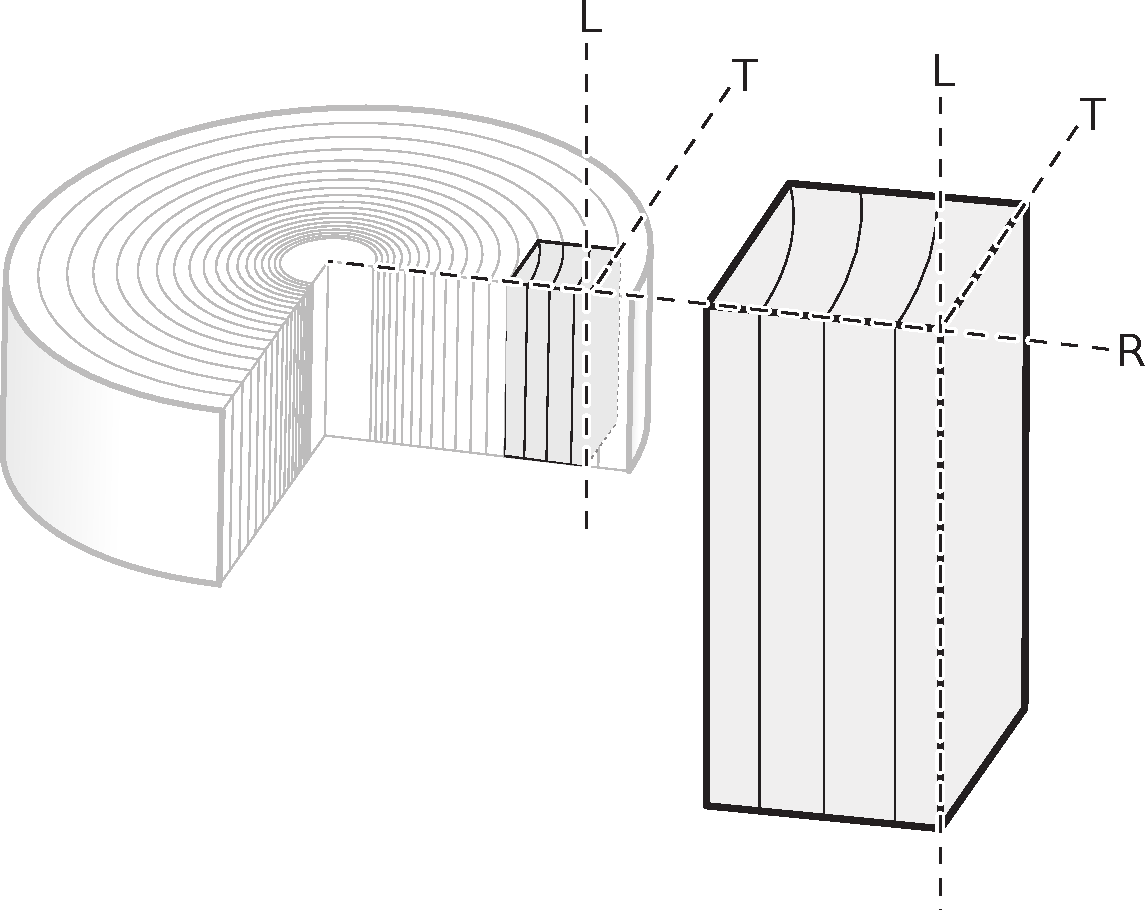
\includegraphics[scale=0.5]{img/ch1_orientation}
\caption{Directions principales et plans principaux du bois. Image préparée par Julie Ferland pour \cite{achim2010dendroecologie}}
\label{plans}
\end{figure}

Les principales structures anatomiques visibles dans chacun des trois plans principaux sont présentées à la Figure~\ref{plansmicro}.

\begin{figure}[p]
\centering

\subfloat[plan transversal]{%
    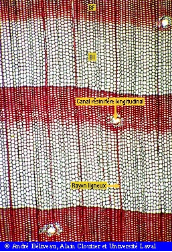
\includegraphics[height=6cm]{img/ch1_transversal}
}
\hfill
\subfloat[Plan longitudinal-tangentiel]{%
	 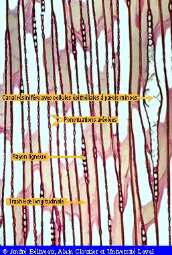
\includegraphics[height=6cm]{img/ch1_longitudinal-tangentiel}
}
\hfill
\subfloat[Plan longitudinal-radial]{%
    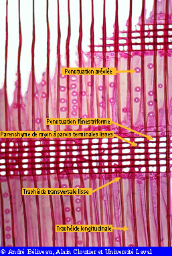
\includegraphics[height=6cm]{img/ch1_longitudinal-radial}
}
\caption{Structures visibles dans chacun des trois plans principaux du bois.}
\label{plansmicro}
\end{figure}